\section{Date: 2026-10-02}
\noindent \textbf{Series ID: PCU6114206114201} 

\noindent This series is titled Producer Price Index by Industry: Computer Training: Computer Training Services and has a frequency of Monthly. The units are Index Jun 2006=100 and the seasonal adjustment is Not Seasonally Adjusted.The observation start date is 2006-06-01 and the observation end date is 2017-08-01.The popularity of this series is 1. \\ 

\noindent \textbf{Series ID: STFAFSXDFBANQ} 

\noindent This series is titled Domestic Finance Companies, Securities, Flow and has a frequency of Quarterly. The units are Millions of Dollars, Quarterly Rate and the seasonal adjustment is Not Seasonally Adjusted.The observation start date is 2011-01-01 and the observation end date is 2026-04-01.The popularity of this series is 1. \\ 

\subsection{Raw Regression}
\noindent Regresses the two series against each other directly. A significant result here can come just as easily from both series sharing a long-run trend as from any real relationship.

\begin{center}
\begin{tabular}{lclc}
\toprule
\textbf{Dep. Variable:}                & value\_fred\_STFAFSXDFBANQ & \textbf{  R-squared:         } &     0.019   \\
\textbf{Model:}                        &            OLS             & \textbf{  Adj. R-squared:    } &    -0.020   \\
\textbf{Method:}                       &       Least Squares        & \textbf{  F-statistic:       } &    0.4905   \\
\textbf{Date:}                         &      Fri, 02 Oct 2026      & \textbf{  Prob (F-statistic):} &    0.490    \\
\textbf{Time:}                         &          16:53:47          & \textbf{  Log-Likelihood:    } &   -262.34   \\
\textbf{No. Observations:}             &               27           & \textbf{  AIC:               } &     528.7   \\
\textbf{Df Residuals:}                 &               25           & \textbf{  BIC:               } &     531.3   \\
\textbf{Df Model:}                     &                1           & \textbf{                     } &             \\
\textbf{Covariance Type:}              &         nonrobust          & \textbf{                     } &             \\
\bottomrule
\end{tabular}
\begin{tabular}{lcccccc}
                                       & \textbf{coef} & \textbf{std err} & \textbf{t} & \textbf{P$> |$t$|$} & \textbf{[0.025} & \textbf{0.975]}  \\
\midrule
\textbf{const}                         &    2.662e+04  &     3.85e+04     &     0.691  &         0.496        &    -5.28e+04    &     1.06e+05     \\
\textbf{value\_fred\_PCU6114206114201} &    -233.6407  &      333.610     &    -0.700  &         0.490        &     -920.724    &      453.443     \\
\bottomrule
\end{tabular}
\begin{tabular}{lclc}
\textbf{Omnibus:}       & 10.482 & \textbf{  Durbin-Watson:     } &    1.690  \\
\textbf{Prob(Omnibus):} &  0.005 & \textbf{  Jarque-Bera (JB):  } &    9.849  \\
\textbf{Skew:}          &  1.008 & \textbf{  Prob(JB):          } &  0.00726  \\
\textbf{Kurtosis:}      &  5.166 & \textbf{  Cond. No.          } & 5.55e+03  \\
\bottomrule
\end{tabular}
%\caption{OLS Regression Results}
\end{center}

Notes: \newline
 [1] Standard Errors assume that the covariance matrix of the errors is correctly specified. \newline
 [2] The condition number is large, 5.55e+03. This might indicate that there are \newline
 strong multicollinearity or other numerical problems.

\begin{figure}
\centering
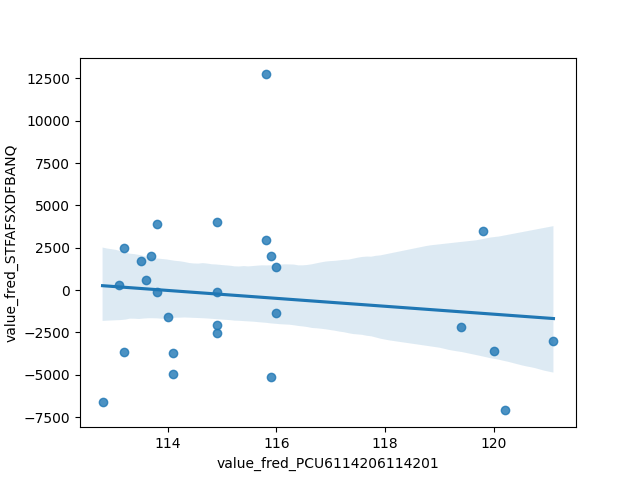
\includegraphics[scale = 0.9]{plots/plot_2026-10-02.png}
\caption{Raw Regression Plot for 2026-10-02}
\end{figure}
\newpage
\subsection{Detrended Regression}
\noindent Regresses the residuals of each series after removing its own linear time trend, so a shared trend can no longer drive the result on its own. A relationship that stays significant here is better evidence of a genuine link between the two series.

\begin{center}
\begin{tabular}{lclc}
\toprule
\textbf{Dep. Variable:}                           & value\_fred\_STFAFSXDFBANQ\_detrended & \textbf{  R-squared:         } &     0.123   \\
\textbf{Model:}                                   &                  OLS                  & \textbf{  Adj. R-squared:    } &     0.088   \\
\textbf{Method:}                                  &             Least Squares             & \textbf{  F-statistic:       } &     3.501   \\
\textbf{Date:}                                    &            Fri, 02 Oct 2026           & \textbf{  Prob (F-statistic):} &   0.0731    \\
\textbf{Time:}                                    &                16:53:47               & \textbf{  Log-Likelihood:    } &   -260.81   \\
\textbf{No. Observations:}                        &                     27                & \textbf{  AIC:               } &     525.6   \\
\textbf{Df Residuals:}                            &                     25                & \textbf{  BIC:               } &     528.2   \\
\textbf{Df Model:}                                &                      1                & \textbf{                     } &             \\
\textbf{Covariance Type:}                         &               nonrobust               & \textbf{                     } &             \\
\bottomrule
\end{tabular}
\begin{tabular}{lcccccc}
                                                  & \textbf{coef} & \textbf{std err} & \textbf{t} & \textbf{P$> |$t$|$} & \textbf{[0.025} & \textbf{0.975]}  \\
\midrule
\textbf{const}                                    &   -1.618e-08  &      758.492     & -2.13e-11  &         1.000        &    -1562.143    &     1562.143     \\
\textbf{value\_fred\_PCU6114206114201\_detrended} &   -1205.5548  &      644.324     &    -1.871  &         0.073        &    -2532.565    &      121.455     \\
\bottomrule
\end{tabular}
\begin{tabular}{lclc}
\textbf{Omnibus:}       &  3.116 & \textbf{  Durbin-Watson:     } &    1.754  \\
\textbf{Prob(Omnibus):} &  0.211 & \textbf{  Jarque-Bera (JB):  } &    1.662  \\
\textbf{Skew:}          &  0.522 & \textbf{  Prob(JB):          } &    0.436  \\
\textbf{Kurtosis:}      &  3.624 & \textbf{  Cond. No.          } &     1.18  \\
\bottomrule
\end{tabular}
%\caption{OLS Regression Results}
\end{center}

Notes: \newline
 [1] Standard Errors assume that the covariance matrix of the errors is correctly specified.

\begin{figure}
\centering
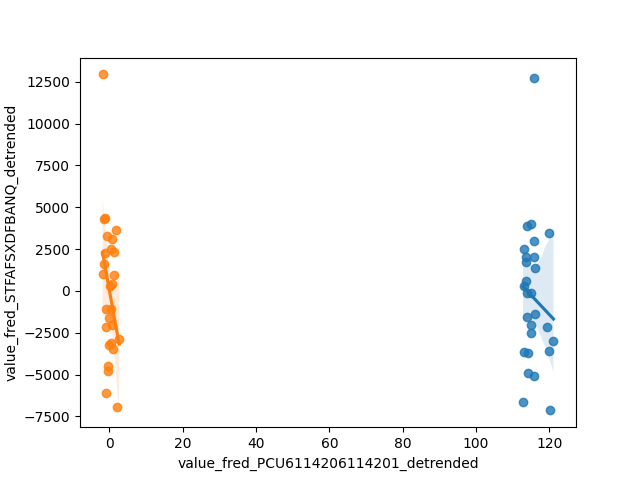
\includegraphics[scale = 0.9]{plots/plot_2026-10-02_detrended.png}
\caption{Detrended Regression Plot for 2026-10-02}
\end{figure}
\newpage
